\documentclass[aspectratio=169]{beamer}
\usepackage[utf8]{inputenc}
\usepackage[T1]{fontenc}
\usepackage[brazil]{babel}
\usepackage{ragged2e}
\usepackage{booktabs}
\usepackage{verbatim}
\usepackage{gensymb}
\usepackage{multirow}
\usepackage{xcolor,colortbl}
\definecolor{verde}{rgb}{0,0.5,0}
\usepackage{listings}
\lstset{
  language=C++,
  basicstyle=\ttfamily,
  keywordstyle=\color{blue},
  stringstyle=\color{verde},
  commentstyle=\color{red},
  extendedchars=true,
  showspaces=false,
  showstringspaces=false,
%  numbers=left,
%  numberstyle=\tiny,
  breaklines=true,
  backgroundcolor=\color{green!10},
  breakautoindent=true,
  captionpos=b,
  xleftmargin=0pt
}
\newcommand\setItemnumber[1]{\setcounter{enumi}{\numexpr#1-1\relax}}

\usetheme{AnnArbor}
\usecolortheme{orchid}
\usefonttheme[onlymath]{serif}

\AtBeginSection[]{
  \begin{frame}
  \vfill
  \centering
  \begin{beamercolorbox}[sep=8pt,center,shadow=true,rounded=true]{title}
    \usebeamerfont{title}\insertsectionhead\par%
  \end{beamercolorbox}
  \vfill
  \end{frame}
}

\title[\sc{Relacionamento entre Classes}]{Relacionamento entre Classes}
\author[Roland Teodorowitsch]{Roland Teodorowitsch}
%\institute[LP2 - EC - PUCRS]{Laboratório de Programação II - Curso de Engenharia de Computação - PUCRS}
\institute[POO - EC - PUCRS]{Programação Orientada a Objetos - ECo - Curso de Engenharia de Computação - PUCRS}
\date{13 de setembro de 2023}

\begin{document}
\justifying

%-------------------------------------------------------
\begin{frame}
	\titlepage
\end{frame}

%=======================================================
\section{Relacionamentos entre Classes}

%-------------------------------------------------------
\begin{frame}\frametitle{Relacionamentos entre Classes}
\begin{itemize}
	\item O que são?
	\begin{itemize}
		\item Os relacionamentos descrevem como as classes interagem umas com as outras
		\item Os relacionamentos entre as classes também definem responsabilidades
	\end{itemize}
	\item Os relacionamentos possuem:
	\begin{itemize}
		\item \textbf{Nome}: descrição dada ao relacionamento (faz, tem, possui, etc.)
		\item \textbf{Sentido de leitura}
		\item \textbf{Navegabilidade}: indicada por uma seta no fim do relacionamento
		\item \textbf{Multiplicidade}: 0..1, 0..*, 1, 1..*, 2, 3..7
		\item \textbf{Tipo}: dependência, associação (agregação, composição) e generalização
		\item \textbf{Papéis}: desempenhados por classes em um relacionamento
	\end{itemize}
\end{itemize}
\end{frame}

%-------------------------------------------------------
\begin{frame}\frametitle{Relacionamentos entre Classes}
\begin{figure}[h]
	\centering
	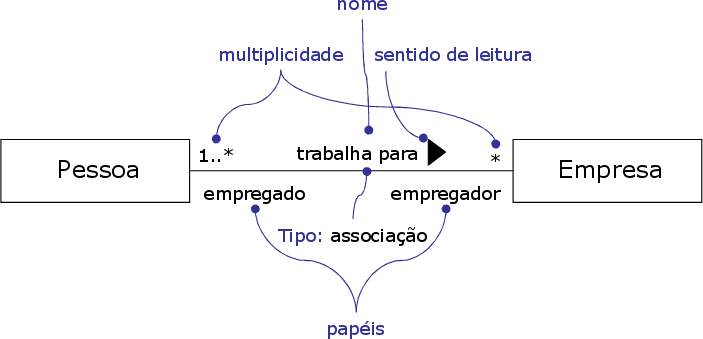
\includegraphics[height=0.32\paperheight]{imagens/relacionamento1.png}
	\end{figure}
\begin{itemize}
	{\small
	\item O cliente sabe quais são seus endereços, mas o endereço não sabe a quais cliente pertence:
		\centering
	\begin{figure}[h]
		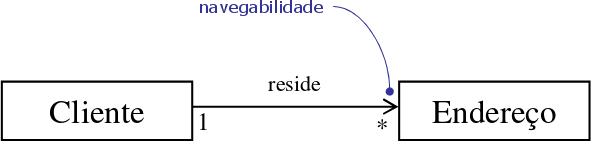
\includegraphics[height=0.12\paperheight]{imagens/relacionamento2.png}
	\end{figure}
	\item Os relacionamentos possíveis entre as classes são: Dependência, Associação, Agregação, Composição e Herança (Generalização/Especialização)
	}
\end{itemize}
\end{frame}

%=======================================================
\section{Dependência}

%-------------------------------------------------------
\begin{frame}\frametitle{Dependência}
\begin{itemize}
	\item Dependência é o relacionamento mais simples entre classes/objetos
	\item A dependência indica que um objeto depende da especificação de outro objeto
	\begin{itemize}
		\item Por especificação, podemos entender a interface pública do objeto (seu conjunto de métodos públicos)
	\end{itemize}
	\item Em um relacionamento de dependência, um objeto é dependente da especificação de outro objeto
	\item Se a especificação mudar, você precisará atualizar o objeto dependente
\end{itemize}
\end{frame}

%-------------------------------------------------------
\begin{frame}\frametitle{Dependência}
\begin{itemize}
	\item A classe A \textbf{depende} da classe B quando:
	\begin{itemize}
		\item A classe A requer a classe B na sua \textbf{especificação} ou \textbf{implementação}
	\end{itemize}
	\item Em UML, a dependência é representada por 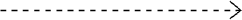
\includegraphics[height=0.025\paperheight]{imagens/dependencia0.png}
	\item Por exemplo:
	\begin{figure}[h]
		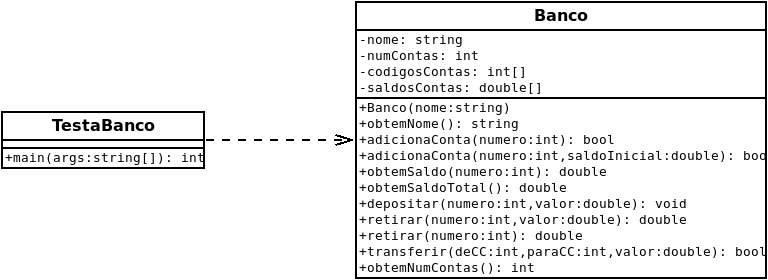
\includegraphics[height=0.4\paperheight]{imagens/dependencia1.png}
	\end{figure}
\end{itemize}
\end{frame}

%-------------------------------------------------------
\begin{frame}\frametitle{Dependência}
\begin{columns}
\begin{column}{0.45\linewidth}
\begin{itemize}
{\small
	\item Quando se deve modelar as dependências?
	\begin{itemize}
{\scriptsize
		\item Para ressaltar grupos de classes relacionadas
		\item Geralmente entre classes importantes
		\item Evitar representação de dependência óbvias
}
	\end{itemize}
	\item Normalmente, se modela dependências quando quer mostrar que um objeto usa outro
	\begin{itemize}
{\scriptsize
		\item Um lugar comum onde um objeto usa outro é através de um argumento de método ou construtor
		\item Por exemplo, o construtor de um objeto da classe Banco recebe um objeto da classe \texttt{string} como argumento.
}
	\end{itemize}
}
\end{itemize}
\end{column}
\begin{column}{0.55\linewidth}
		\begin{figure}[h]
			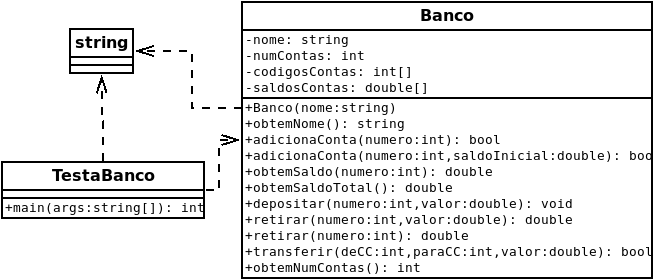
\includegraphics[height=0.35\paperheight]{imagens/dependencia2.png}
		\end{figure}
\end{column}
\end{columns}
\end{frame}

%=======================================================
\section{Associação}

%-------------------------------------------------------
\begin{frame}\frametitle{Associação}
\begin{itemize}
	\item Os relacionamentos de associação vão um pouco mais fundo do que os relacionamentos de dependência
	\item As associações representam relação entre objetos
	\item As associações são relacionamentos estruturais
	\item Uma associação indica que um objeto \textbf{contém (ou que está conectado a)} outro objeto
\end{itemize}
\end{frame}

%-------------------------------------------------------
\begin{frame}\frametitle{Associação}
\begin{itemize}
	\item A classe A \textbf{tem associação X} com a classe B
	\begin{itemize}
		\item Objetos da classe A tem relacionamento X com objetos da classe B
	\end{itemize}
	\item Em UML, a associação é representada por 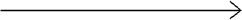
\includegraphics[height=0.025\paperheight]{imagens/associacao0.png}
	\item Por exemplo:
\begin{columns}
\begin{column}{0.5\linewidth}
	\begin{figure}[h]
		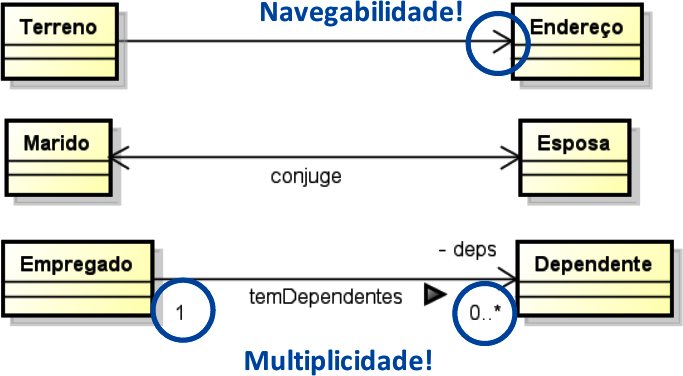
\includegraphics[height=0.4\paperheight]{imagens/associacao1.png}
	\end{figure}
\end{column}
\begin{column}{0.5\linewidth}
	\begin{figure}[h]
		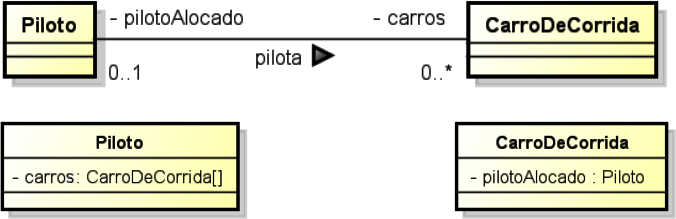
\includegraphics[height=0.25\paperheight]{imagens/associacao2.png}
	\end{figure}
\end{column}
\end{columns}
\end{itemize}
\end{frame}

%-------------------------------------------------------
\begin{frame}[fragile]\frametitle{Relações 1:1}
\begin{columns}
\begin{column}{0.5\linewidth}
	\begin{figure}[h]
		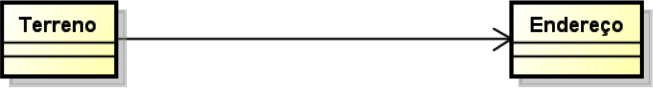
\includegraphics[height=0.1\paperheight]{imagens/associacao3.png}
	\end{figure}
\begin{lstlisting}[language=C++]
class Terreno {
private:
  Endereco endereco;
  ...
};



class Endereco {
  ...
};
\end{lstlisting}

\end{column}
\begin{column}{0.5\linewidth}
	\begin{figure}[h]
		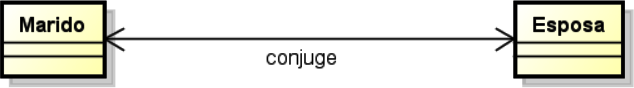
\includegraphics[height=0.1\paperheight]{imagens/associacao4.png}
	\end{figure}

\begin{lstlisting}[language=C++]
class Marido {
private:
  Esposa *conjuge;
  ...
};

class Esposa {
private:
  Marido *conjuge;
  ...
};
\end{lstlisting}
\end{column}
\end{columns}
\end{frame}

%-------------------------------------------------------
\begin{frame}[fragile]\frametitle{Relações 1:n}
\begin{figure}[h]
	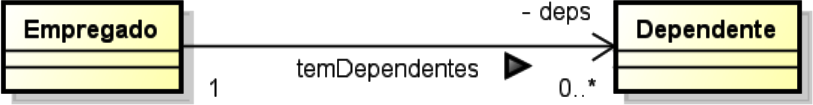
\includegraphics[height=0.1\paperheight]{imagens/associacao5.png}
\end{figure}
\begin{lstlisting}[language=C++]
class Empregado {
private:
  Dependente deps[N];
  ...
};

class Dependente {
  ...
};
\end{lstlisting}
\end{frame}

%-------------------------------------------------------
\begin{frame}\frametitle{Associação}
\begin{columns}
\begin{column}{0.5\linewidth}
\begin{itemize}
	\item Quando você deve modelar associações?
	\begin{itemize}
		\item Você deve modelar associações quando um objeto contiver outro objeto (o relacionamento ``tem um'')
		\item Você também pode modelar uma associação quando um objeto usa outro
		\item Uma associação permite que você modele quem faz o que em um relacionamento
	\end{itemize}
	\item Para refinar ainda mais os modelos, UML define dois tipos de associação: agregação e composição
\end{itemize}
\end{column}
\begin{column}{0.5\linewidth}
		\begin{figure}[h]
			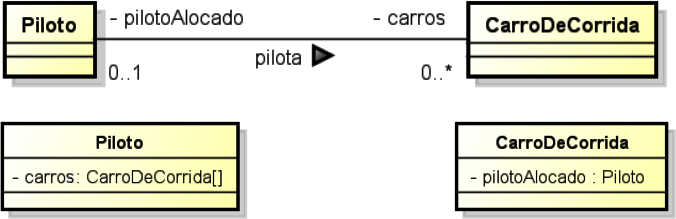
\includegraphics[height=0.25\paperheight]{imagens/associacao2.png}
		\end{figure}
\end{column}
\end{columns}
\end{frame}

%=======================================================
\section{Agregação}

%-------------------------------------------------------
\begin{frame}\frametitle{Agregação}
\begin{itemize}
	\item Uma agregação é um tipo especial de associação
	\item Uma agregação modela um relacionamento \textbf{tem um} (ou \textbf{parte de}) entre pares
	\item Esse relacionamento significa que \textbf{um objeto NÃO é mais importante do que o outro}
	\item Importância, no contexto de agregação, significa que os objetos podem existir independentemente uns dos outros
	\item Isto é, se o objeto deixa de existir, os outros objetos que fazem parte do modelo podem continuar existindo
\end{itemize}
\begin{figure}[h]
	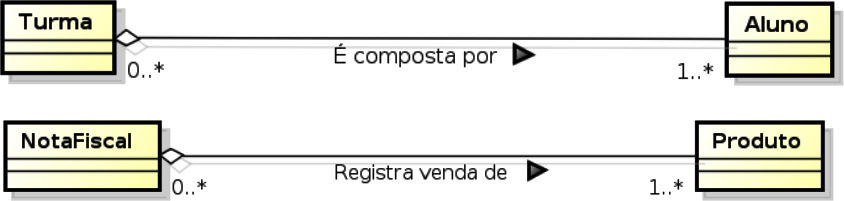
\includegraphics[height=0.25\paperheight]{imagens/agregacao.png}
\end{figure}
\end{frame}

%=======================================================
\section{Composição}

%-------------------------------------------------------
\begin{frame}\frametitle{Composição}
\begin{itemize}
	\item A composição é um pouco mais rigorosa do que a agregação
	\item A composição não é um relacionamento entre pares. Os objetos não são independentes uns dos outros
	\item Isso significa, em termos de programação, que quando o objeto todo é destruído, todos os objetos parte são automaticamente destruídos também
\end{itemize}
\begin{figure}[h]
	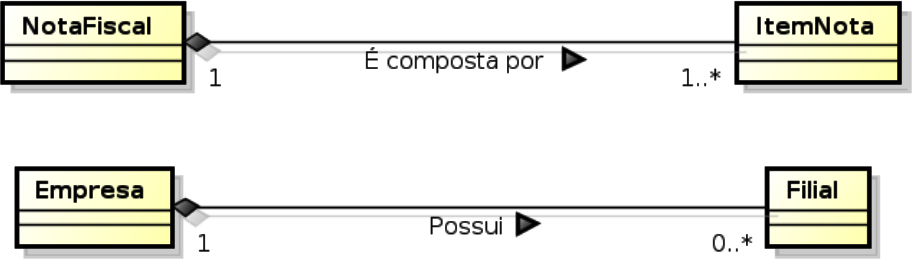
\includegraphics[height=0.25\paperheight]{imagens/composicao.png}
\end{figure}
\end{frame}

%=======================================================
\section{Aplicando Relacionamento entre Classes na Classe Banco}

%-------------------------------------------------------
\begin{frame}\frametitle{Classe Banco}
\begin{figure}[h]
	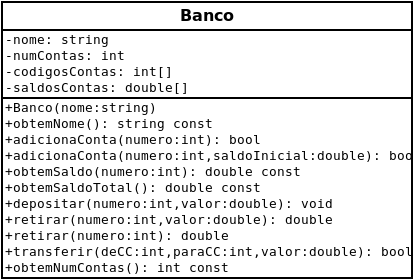
\includegraphics[height=0.6\paperheight]{imagens/banco1.png}
\end{figure}
\end{frame}

%-------------------------------------------------------
\begin{frame}\frametitle{Classe Banco com Classe Conta}
\begin{figure}[h]
	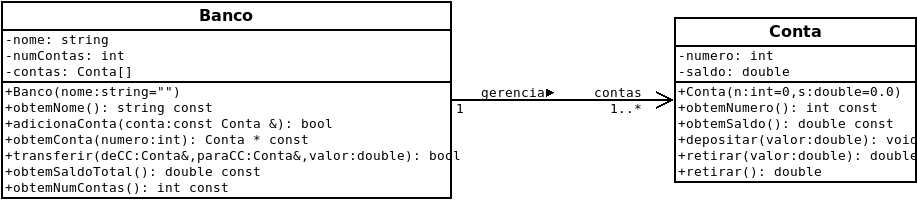
\includegraphics[height=0.35\paperheight]{imagens/banco2.png}
\end{figure}
\end{frame}

%-------------------------------------------------------
\begin{frame}[fragile]\frametitle{Classe Banco em C++}
\begin{lstlisting}[language=C++,basicstyle=\ttfamily\tiny]
class Banco {
private:
  string nome;
  Conta contas[N];
  int numContas;
public:

  Banco(string nome){
    this->nome = nome;
    numContas = 0;
  }

  ...

  bool adicionaConta(const Conta &c){
    if (numContas < N){
       contas[numContas] = c;
       numContas++;
       return true;
    }
    return false;
  }

  ...
};
\end{lstlisting}
\end{frame}

%-------------------------------------------------------
\begin{frame}\frametitle{Associações e Dependências}
\begin{itemize}
	\item Associações:
	\begin{itemize}
		\item Normalmente mapeiam para atributos
	\end{itemize}
	\item Atributo x Associação:
	\begin{itemize}
		\item Convenção:
		\begin{itemize}
			\item Atributos para classes são associações
			\item Atributos para tipos primitivos não
		\end{itemize}
		\item Quando usar no caso de classes:
		\begin{itemize}
			\item Modelo compacto: atributos
			\item Ressaltar relacionamento: associação
		\end{itemize}
	\end{itemize}
	\item Dependência x Associação:
	\begin{itemize}
		\item Associação comumente implica em dependência
	\end{itemize}
\end{itemize}
\end{frame}

%=======================================================
\section{Exercício}

%-------------------------------------------------------
\begin{frame}\frametitle{Exercício}
\begin{enumerate}
	\item Reimplemente Banco segundo o diagrama abaixo:
\begin{figure}[h]
	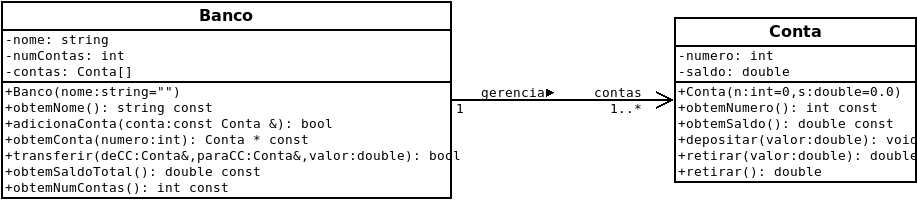
\includegraphics[height=0.34\paperheight]{imagens/banco2.png}
\end{figure}
	\item Faça um programa principal para testar os métodos das classes.
\end{enumerate}
\end{frame}

%=======================================================
\section{Créditos}

%-------------------------------------------------------
\begin{frame}\frametitle{Créditos}
\begin{itemize}
	\item Estas lâminas contêm trechos de materiais disponibilizados pelos professores Rafael Garibotti, Daniel Callegari, Sandro Fiorini e Bernardo Copstein.
\end{itemize}
\end{frame}

%=======================================================
\section{Soluções}

%-------------------------------------------------------
\begin{frame}[fragile]\frametitle{Exercício 1: \texttt{Conta.hpp}}
\fontsize{6pt}{6pt}\selectfont{
\lstinputlisting{src/Conta.hpp}
}
\end{frame}

%-------------------------------------------------------
\begin{frame}[fragile]\frametitle{Exercício 1: \texttt{Conta.cpp}}
\fontsize{5pt}{5pt}\selectfont{
\lstinputlisting{src/Conta.cpp}
}
\end{frame}

%-------------------------------------------------------
\end{document}

